
%%%%%%%%%%%%%%%%%%%%%%%%%%%%%%%%%%%%%%%%%%%%%%%%%%%%%%%%%%%%%%%%%%%%%%%%%%%%%%%%%%%%%%%
%%%%%%%%%%%%%%%%%%%%%%%%%%%%%%%%%%%%%%%%%%%%%%%%%%%%%%%%%%%%%%%%%%%%%%%%%%%%%%%%%%%%%%%
% 
% This top part of the document is called the 'preamble'.  Modify it with caution!
%
% The real document starts below where it says 'The main document starts here'.

\documentclass[12pt]{article}

\usepackage{amssymb,amsmath,amsthm}
\usepackage[top=1in, bottom=1in, left=1.25in, right=1.25in]{geometry}
\usepackage{fancyhdr}
\usepackage{enumerate}
\usepackage{listings}
\usepackage{graphicx}
\usepackage{float}

% Comment the following line to use TeX's default font of Computer Modern.
\usepackage{times,txfonts}



\makeatletter
\renewcommand*\env@matrix[1][*\c@MaxMatrixCols c]{%
  \hskip -\arraycolsep
  \let\@ifnextchar\new@ifnextchar
  \array{#1}}
\makeatother

\newtheoremstyle{homework}% name of the style to be used
  {18pt}% measure of space to leave above the theorem. E.g.: 3pt
  {12pt}% measure of space to leave below the theorem. E.g.: 3pt
  {}% name of font to use in the body of the theorem
  {}% measure of space to indent
  {\bfseries}% name of head font
  {:}% punctuation between head and body
  {2ex}% space after theorem head; " " = normal interword space
  {}% Manually specify head
\theoremstyle{homework} 

% Set up an Exercise environment and a Solution label.
\newtheorem*{exercisecore}{Exercise \@currentlabel}
\newenvironment{exercise}[1]
{\def\@currentlabel{#1}\exercisecore}
{\endexercisecore}

\newcommand{\localhead}[1]{\par\smallskip\noindent\textbf{#1}\nobreak\\}%
\newcommand\solution{\localhead{Solution:}}

%%%%%%%%%%%%%%%%%%%%%%%%%%%%%%%%%%%%%%%%%%%%%%%%%%%%%%%%%%%%%%%%%%%%%%%%
%
% Stuff for getting the name/document date/title across the header
\makeatletter
\RequirePackage{fancyhdr}
\pagestyle{fancy}
\fancyfoot[C]{\ifnum \value{page} > 1\relax\thepage\fi}
\fancyhead[L]{\ifx\@doclabel\@empty\else\@doclabel\fi}
\fancyhead[C]{\ifx\@docdate\@empty\else\@docdate\fi}
\fancyhead[R]{\ifx\@docauthor\@empty\else\@docauthor\fi}
\headheight 15pt

\def\doclabel#1{\gdef\@doclabel{#1}}
\doclabel{Use {\tt\textbackslash doclabel\{MY LABEL\}}.}
\def\docdate#1{\gdef\@docdate{#1}}
\docdate{Use {\tt\textbackslash docdate\{MY DATE\}}.}
\def\docauthor#1{\gdef\@docauthor{#1}}
\docauthor{Use {\tt\textbackslash docauthor\{MY NAME\}}.}
\makeatother

% Shortcuts for blackboard bold number sets (reals, integers, etc.)
\newcommand{\Reals}{\ensuremath{\mathbb R}}
\newcommand{\Nats}{\ensuremath{\mathbb N}}
\newcommand{\Ints}{\ensuremath{\mathbb Z}}
\newcommand{\Rats}{\ensuremath{\mathbb Q}}
\newcommand{\Cplx}{\ensuremath{\mathbb C}}
%% Some equivalents that some people may prefer.
\let\RR\Reals
\let\NN\Nats
\let\II\Ints
\let\CC\Cplx

%%%%%%%%%%%%%%%%%%%%%%%%%%%%%%%%%%%%%%%%%%%%%%%%%%%%%%%%%%%%%%%%%%%%%%%%%%%%%%%%%%%%%%%
%%%%%%%%%%%%%%%%%%%%%%%%%%%%%%%%%%%%%%%%%%%%%%%%%%%%%%%%%%%%%%%%%%%%%%%%%%%%%%%%%%%%%%%
% 
% The main document start here.

% The following commands set up the material that appears in the header.
\doclabel{STAT 402: Homework 3}
\docauthor{Stefano Fochesatto}
\docdate{\today}

\begin{document}

\begin{exercise}{1} Consider the data table from problem 9 in the last homework.
    \begin{enumerate}[a.]
        \item Take a SRS of size $n = 8$ from the top three rows, then another sample
        of size $n = 10$ from the bottom four rows. Then use stratified sampling estimator to get an 
        estimate of the total over the entire region. \\
        \solution
        \textbf{Code:}
        \begin{center}
            \lstinputlisting{r1.txt}
        \end{center}

        \item How does the confidence interval in $a$ compare to the one in the last homework?
        In particular, how wide are the intervals? Why do you think this occurred?\\
        \solution Given that the standard error I from the simple random sample in problem 9 is actually
        smaller than the stratified sample above, the confidence interval was actually smaller before, without stratification. 
        I think this can possibly be attributed to a poor grouping of strata that don't actually minimize the variance. 
    \end{enumerate}
\end{exercise}
\vspace{1in}


\begin{exercise}{2} I want to know the average contamination level in a plot of ground. 
    Just by looking at the area, I see that part has discolored soil and damaged plats. I'll put 
    this area into one stratum and the rest of the area into another stratum. \\
    I collect $n = 3$ measurements in each stratum:\\
    Stratum One (appears contaminated): $Area = 5$ Hectares, $Measurements = [50, 100 ,75]$ ppt\\
    Stratum Two (appears uncontaminated): $Area = 45$ Hectares, $Measurements = [1, 3 ,2]$ ppt\\
    
    \begin{enumerate}
        \item Find a 95 percent confidence interval for the true mean contamination level.\\
        \solution  
        \textbf{Code:}
        \begin{center}
            \lstinputlisting{r2.txt}
        \end{center}
        \vspace{.15in}

        \item Assuming the cost of collecting data is the same everywhere, use the 
        variances from the study to plan next year's study, with the goal of getting an optimal 
        allocation with margin of 1ppt.\\
        \solution With constant cost, the equation for computing optimal allocation simplifies to, 
        \begin{equation*}
            w_i = \dfrac{N_i \sigma_i}{\sum_{j = i}^K N_j\sigma_j}
        \end{equation*} 
        \textbf{Code:}
        \begin{center}
            \lstinputlisting{r3.txt}
        \end{center}
        \vspace{.15in}
    \end{enumerate}
\end{exercise}
\vspace{1in}


\begin{exercise}{3} We wish to find the proportion of people who support a candidate in an election.
    We could use a $SRS$ over the entire city, but instead we know one area ($N_1 = 12000$ voters) where
    our candidate isn't very popular(less than 30 percent is our guess) and another area ($N_2 = 24000$ voters)
    where we think or candidate will be more popular (over 50 percent, as a guess). We perform a SRS
    in stratum and get the following:\\
    Stratum One: $N_1 = 12000$, $p_1 = .25$, $n_1 = 200$. \\
    Stratum Two: $N_2 = 24000$, $p_2 = .65$, $n_2 = 400.4$.\\
    \begin{enumerate}[a.]
        \item Find a 95 percent confidence interval for the true proportion over the entire city.\\
        \solution 
        \textbf{Code:}
        \begin{center}
            \lstinputlisting{r4.txt}
        \end{center}
        \vspace{.15in}

        \item Is this proportional allocation? Why or why not? If so, why did I use proportional allocation?
        If not, why did I choose the sample sizes I did?\\
        \solution This is an example of proportional allocation. We can see that the sample sizes were chosen
        as a proportionally with respect to the size of the stratum. Proportional allocation gives an unbiased estimator 
        when the true proportion or even an estimate isn't had to compute the optimal allocation. 
        \vspace{.15in}


        \item Was stratification a good idea in this case? Why or why not?\\
        \solution Computing the estimated proportion as one SRS we can find out if stratifying reduced 
        the SE in any useful way.\\
        \textbf{Code:}
        \begin{center}
            \lstinputlisting{r6.txt}
        \end{center}
        From the code we can see that the SE was reduced $~.2\%$, when we stratified. In general we should 
        see a reduction in the SE when stratum proportions $\hat{p_i}$ are more ideal than $.50$. Elections have been 
        won on margins less than $.04\%$ so I would say stratification is a good idea in this case. 
    \end{enumerate}
\end{exercise}
\vspace{1in}


\begin{exercise}{4} For the results in problem 3, if we had known the proportions were around
    $.25$ and $.65$, what would be the optimal allocation of the sample between the two strata?
    If we wanted a bound of $\pm .05$, what sample size should I take. (Assuming constant cost)\\
    \solution 
    \textbf{Code:}
        \begin{center}
            \lstinputlisting{r5.txt}
        \end{center}
\end{exercise}
\vspace{1in}


\begin{exercise}{5} We get to see an entire population once again. Yep, that happens
    a lot in practice... We want to take a total sample of size $n = 9$ from the population of 
    $N = 40$ equal-area plots. We want to estimate the total grass cover in the region. Measuring
    that is not easy, but it is easy to quickly look over the plots and 'guess' at the grass cover.
    below is the real population(which we magically see) along with the 'guess' at grass cover, which we 
    do know for all of the plots.\\
    In other words, start by pretending that you can't see the second column. the use then use these values
    to divide the plot into strata. Finally, you will take a sample in each of the strata, where you can 
    write down the value of the second column for the plots you sample.\\
    \begin{enumerate}[a.]
        \item In reality, you only know the guess until you take your sample. Use the guesses to stratify
        the population into three strata. Tell me how you decided upon a sample size for each. Then use a 
        randomization method to select three plots from each stratum. Then write down the 'true cover'
        for those plots.\\
        \solution To group the plots up into strata I simply plotted a histogram with the minimal number of 
        bins possible. Doing so gave me this histogram,
        \begin{figure}[H]
            \begin{center}
            \caption{Histogram of the guess cover.}
            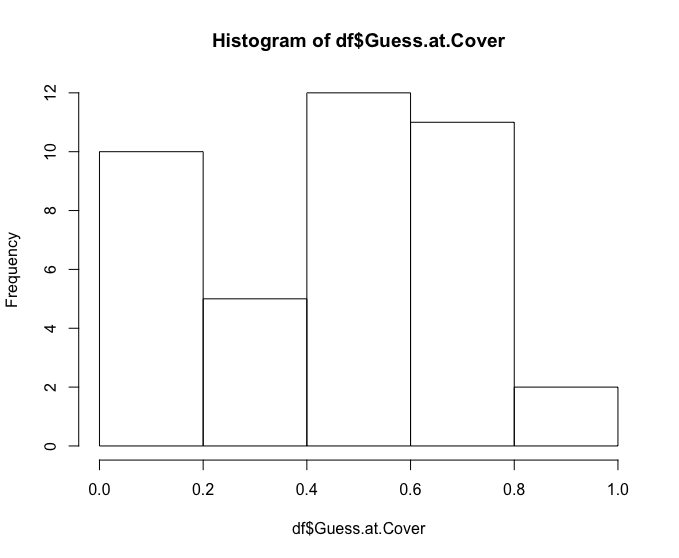
\includegraphics[width=.70\textwidth]{Rplot01.png}
            \end{center}
        \end{figure}
        Looking at the histogram I decided to group the strata with the following criteria,\\
        \textbf{Code:}
        \begin{center}
            \lstinputlisting{r7.txt}
        \end{center}
        \vspace{.15in}


        \item With the data from $a.$ find the 95 percent confidence interval for the mean cover. \\
        \solution 
        \textbf{Code:}
        \begin{center}
            \lstinputlisting{r8.txt}
        \end{center}
        Looking at the confidence interval, we can see that we do contain the true mean cover, and our estimate
        is also within 1 standard error. 
    \end{enumerate}
    
\end{exercise}











\end{document}




















